\chapter{EtherChannel}\label{etherchannel}

WHAT IS ETHERCHANNEL?

ETHERCHANNEL allows you to GROUP multiple physical INTERFACES into a
group which operates as a SINGLE LOGICAL INTERFACE - so they BEHAVE as
if they are a single INTERFACE

A LAYER 2 ETHERCHANNEL is a group of SWITCH PORTS which operate as a
SINGLE INTERFACE

A LAYER 3 ETHERCHANNEL is a group of ROUTED PORTS which operate as a
SINGLE INTERFACE which you assign an IP ADDRESS to.

\begin{figure}
\centering
\pandocbounded{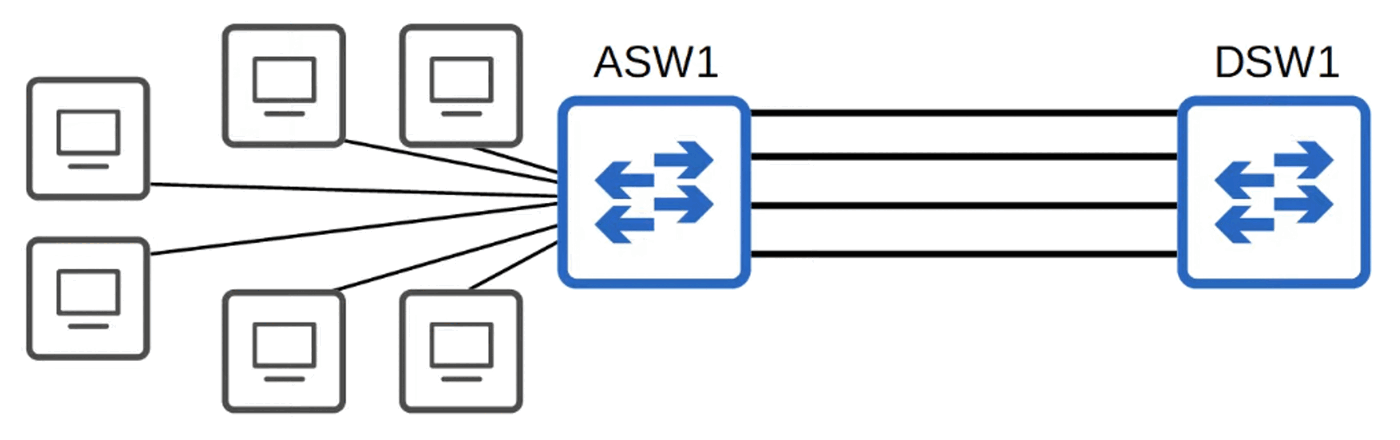
\includegraphics[keepaspectratio,alt={image}]{images/24-etherchannel/img-001.png}}
\end{figure}

When the bandwidth of the INTERFACES connected to END HOSTS is greater
than the bandwidth of the connection to the DISTRIBUTION SWITCH(es),
this is called \textbf{OVERSUBSCRIPTION.}

Some OVERSUBSCRIPTION is acceptable, but too much will cause congestion.

\begin{figure}
\centering
\pandocbounded{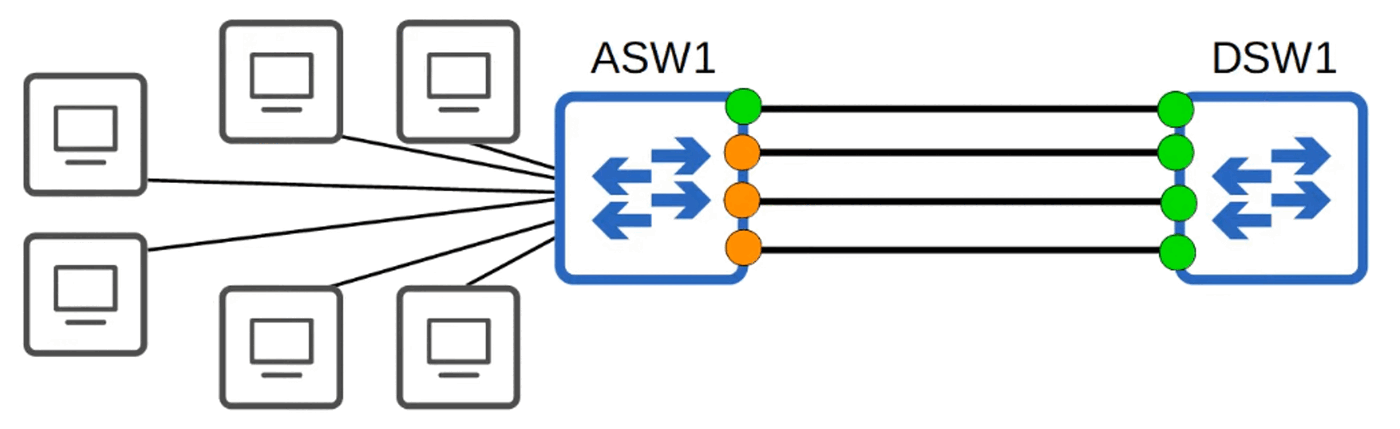
\includegraphics[keepaspectratio,alt={image}]{images/24-etherchannel/img-002.png}}
\end{figure}

\begin{itemize}
\tightlist
\item
  If you connect TWO SWITCHES together with multiple links, ALL except
  ONE will be DISABLED by SPANNING TREE PROTOCOL (Green Lights
  vs.~Orange Lights above on ASW1)
\end{itemize}

WHY?

\begin{itemize}
\tightlist
\item
  If ALL of ASW1s INTERFACES were FORWARDING, LAYER 2 LOOPS would form
  between ASW1 and DSW1, leading to a BROADCAST STORM (Bad!)
\item
  Other links will be unused unless the active link fails. In that case,
  one of the inactive link will start forwarding.
\end{itemize}

An ETHERCHANNEL (in network topology diagrams) is represented like THIS
(circle around multi-connections)

\begin{figure}
\centering
\pandocbounded{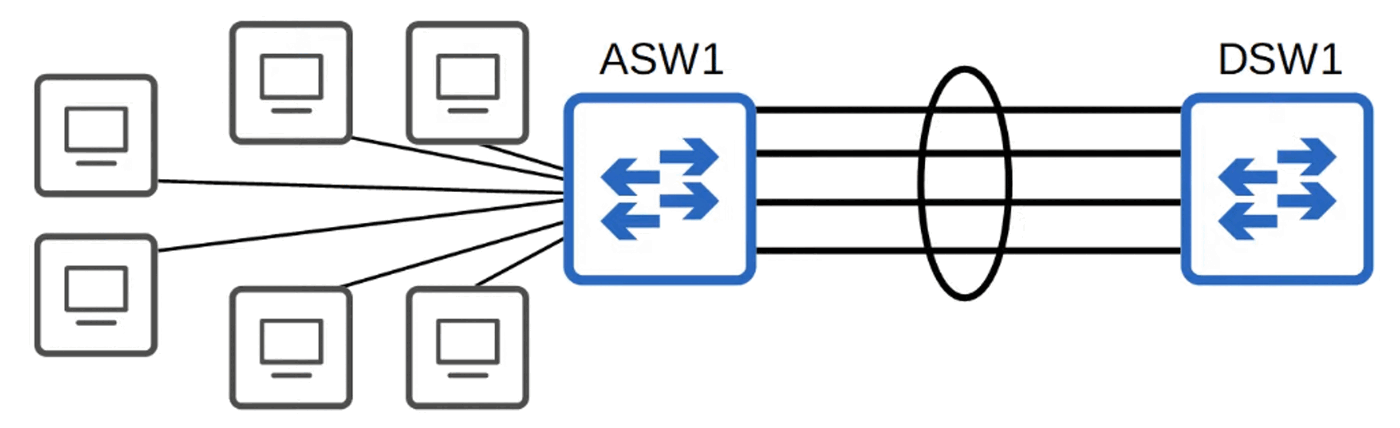
\includegraphics[keepaspectratio,alt={image}]{images/24-etherchannel/img-003.png}}
\end{figure}

\begin{itemize}
\tightlist
\item
  ETHERCHANNEL groups multiple channels together to act as a SINGLE
  INTERFACE
\item
  STP will treat this GROUP as a SINGLE INTERFACE
\end{itemize}

\begin{figure}
\centering
\pandocbounded{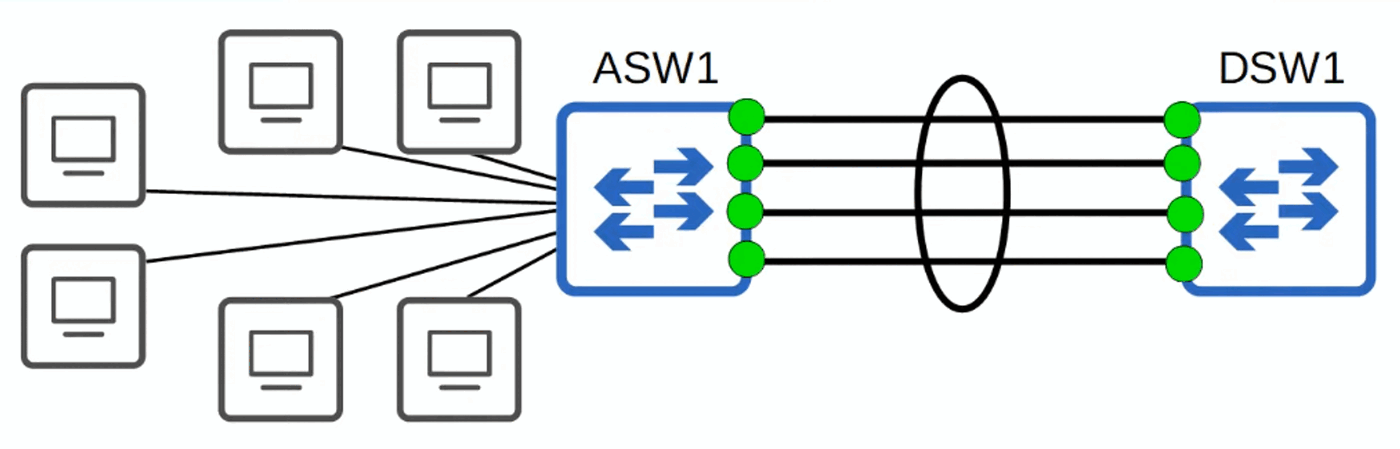
\includegraphics[keepaspectratio,alt={image}]{images/24-etherchannel/img-004.png}}
\end{figure}

(All INTERFACES Green!)

TRAFFIC using ETHERCHANNEL will be load-balanced among the physical
INTERFACES in the group.

An algorithm is used to determine WHICH TRAFFIC will use WHICH physical
INTERFACE (more details later)

Some other names for an ETHERCHANNEL are:

\begin{itemize}
\tightlist
\item
  PORT CHANNEL
\item
  LAG (Link Aggregation Group)
\end{itemize}

HOW DOES AN ETHERCHANNEL LOAD-BALANCE?

\begin{figure}
\centering
\pandocbounded{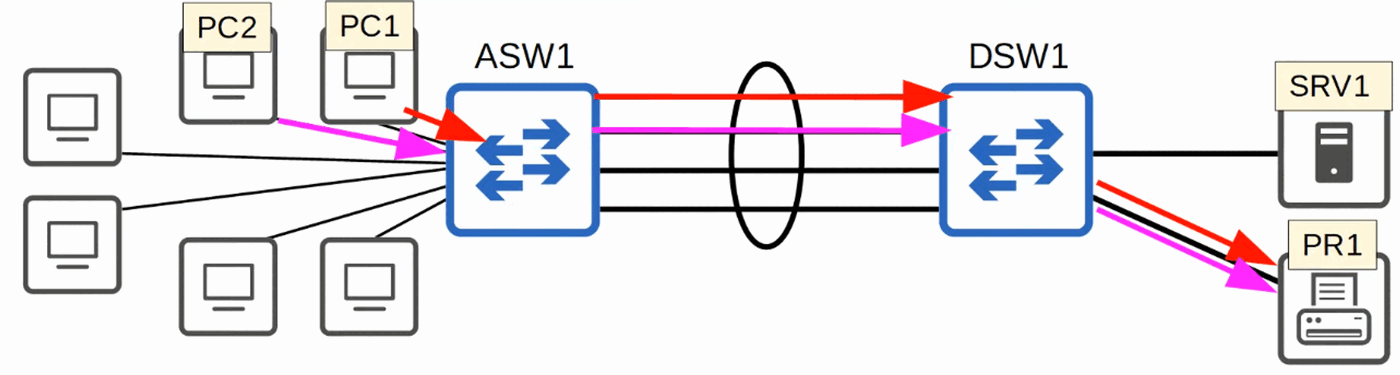
\includegraphics[keepaspectratio,alt={image}]{images/24-etherchannel/img-005.png}}
\end{figure}

\begin{itemize}
\tightlist
\item
  ETHERCHANNEL load-balances based on \textbf{``flows''}
\item
  A ``flow'' is a communication between TWO NODES in the NETWORK
\item
  FRAMES in the same ``flow'' will be FORWARDED using the SAME physical
  INTERFACE
\item
  If FRAMES in the same ``flow'' were FORWARDED using different physical
  INTERFACES, some FRAMES may arrive at the DESTINATION out of
  order/sequence, which can cause problems.
\item
  You can CHANGE the INPUTS used in the INTERFACE SELECTION calculation
  (for ``flows'')

  \begin{itemize}
  \tightlist
  \item
    INPUTS that can be used:

    \begin{itemize}
    \tightlist
    \item
      SOURCE MAC ADDRESS
    \item
      DESTINATION MAC ADDRESS
    \item
      SOURCE and DESTINATION MAC ADDRESS
    \item
      SOURCE IP ADDRESS
    \item
      DESTINATION IP ADDRESS
    \item
      SOURCE and DESTINATION IP ADDRESS
    \end{itemize}
  \end{itemize}
\end{itemize}

How to see the configuration for LOAD-BALANCING method

\begin{figure}
\centering
\pandocbounded{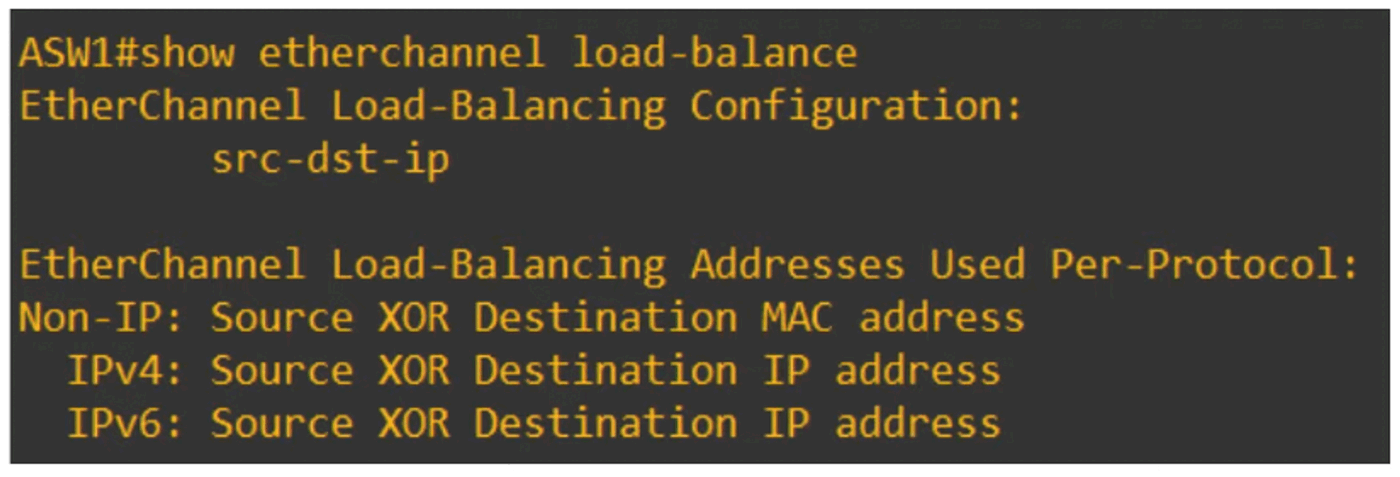
\includegraphics[keepaspectratio,alt={image}]{images/24-etherchannel/img-006.png}}
\end{figure}

How to CHANGE the LOAD-BALANCING method

\begin{figure}
\centering
\pandocbounded{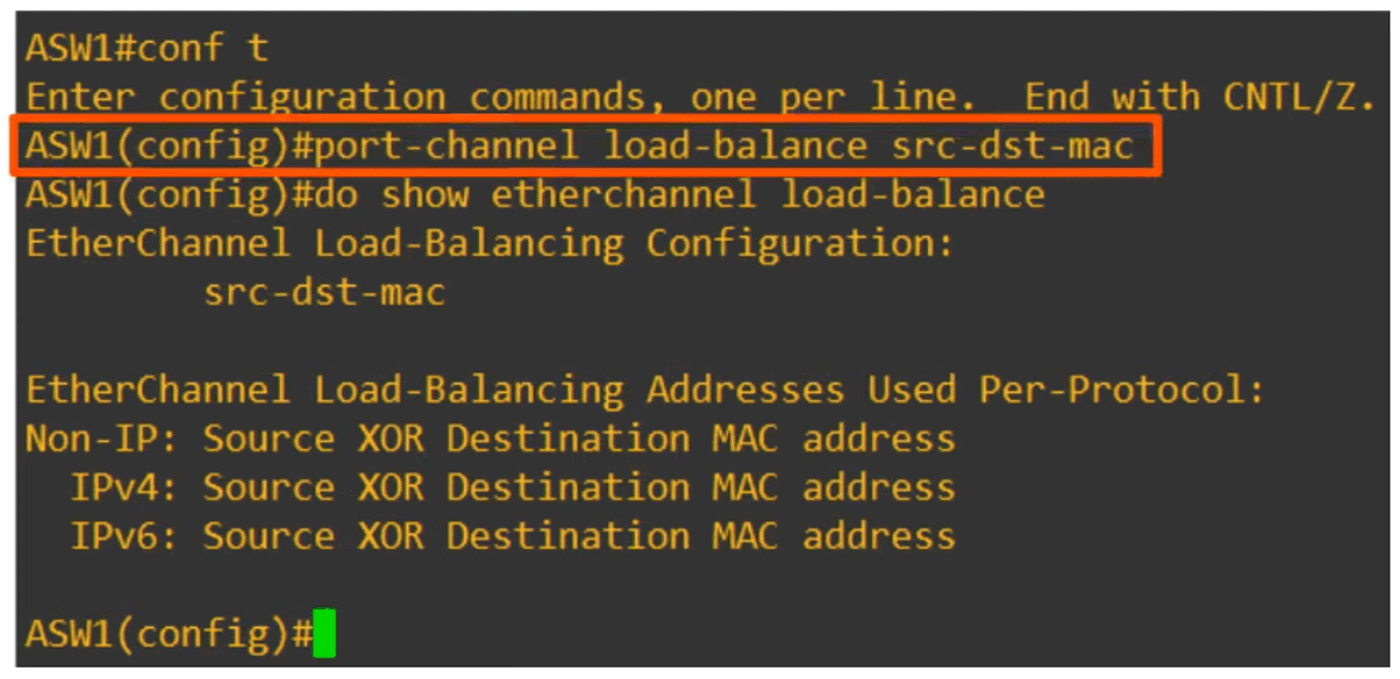
\includegraphics[keepaspectratio,alt={image}]{images/24-etherchannel/img-007.png}}
\end{figure}

\begin{figure}
\centering
\pandocbounded{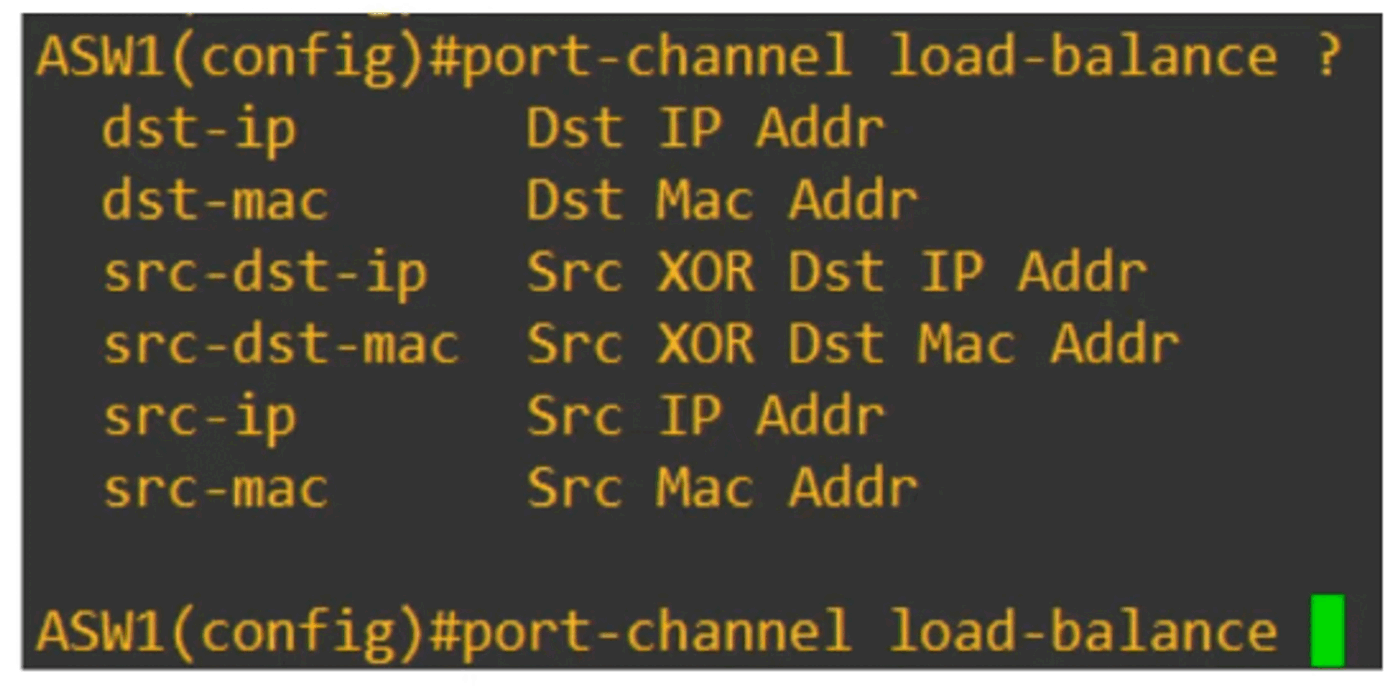
\includegraphics[keepaspectratio,alt={image}]{images/24-etherchannel/img-008.png}}
\end{figure}

\section{How to Configure Layer 2 / Layer 3
EtherChannels}\label{how-to-configure-layer-2-layer-3-etherchannels}

There are THREE methods of ETHERCHANNEL configuration on Cisco SWITCHES

\textbf{PAgP (Port Aggregation Protocol)}

\begin{itemize}
\tightlist
\item
  Cisco proprietary protocol
\item
  Dynamically negotiates the creation/maintenance of the ETHERCHANNEL
  (like DTP does for trunks)
\end{itemize}

\textbf{LACP (Link Aggregation Control Protocol)} - Industry standard
protocol (IEEE 802.3ad) - Dynamically negotiates the
creation/maintenance of the ETHERCHANNEL (like DTP does for trunks)

\textbf{Static EtherChannel}

\begin{itemize}
\tightlist
\item
  A protocol isn't used to determine if an EtherChannel should be formed
\item
  Interfaces are statically configured to form an EtherChannel
\end{itemize}

Up to 8 INTERFACES can be formed into a single ETHERCHANNEL (LACP allows
up to 16 but only 8 will be ACTIVE, the other 8 will in STANDBY mode,
waiting for an active INTERFACE to fail)

PAgP CONFIGURATION

\begin{figure}
\centering
\pandocbounded{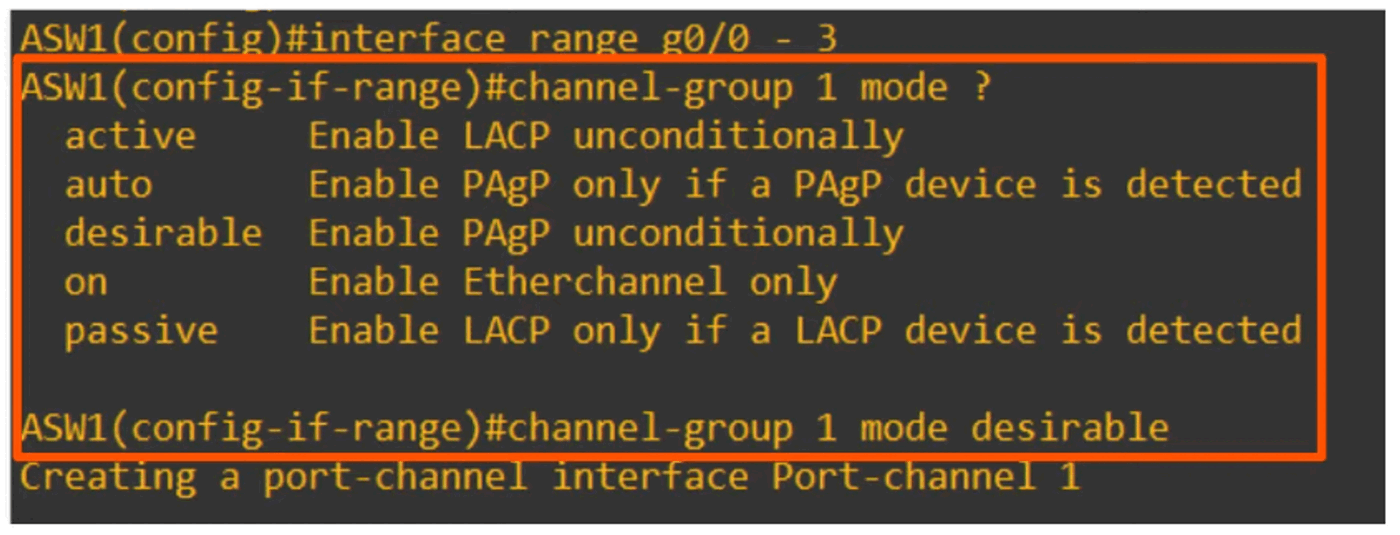
\includegraphics[keepaspectratio,alt={image}]{images/24-etherchannel/img-009.png}}
\end{figure}

NOTE that ``auto'' and ``desirable'' are the ONLY available modes for
PAgP

\begin{figure}
\centering
\pandocbounded{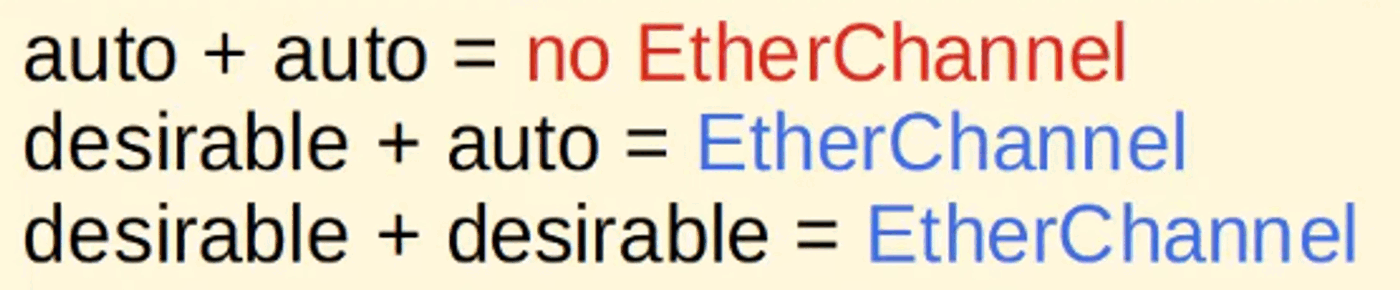
\includegraphics[keepaspectratio,alt={image}]{images/24-etherchannel/img-010.png}}
\end{figure}

PAgP negotiations to form an ETHERCHANNEL

AWS1(config-if-range)\# channel-group 1 mode desirable. Creating a
port-channel interface Port-channel1

Shows up in the interface as ``Port-channel1''

\begin{figure}
\centering
\pandocbounded{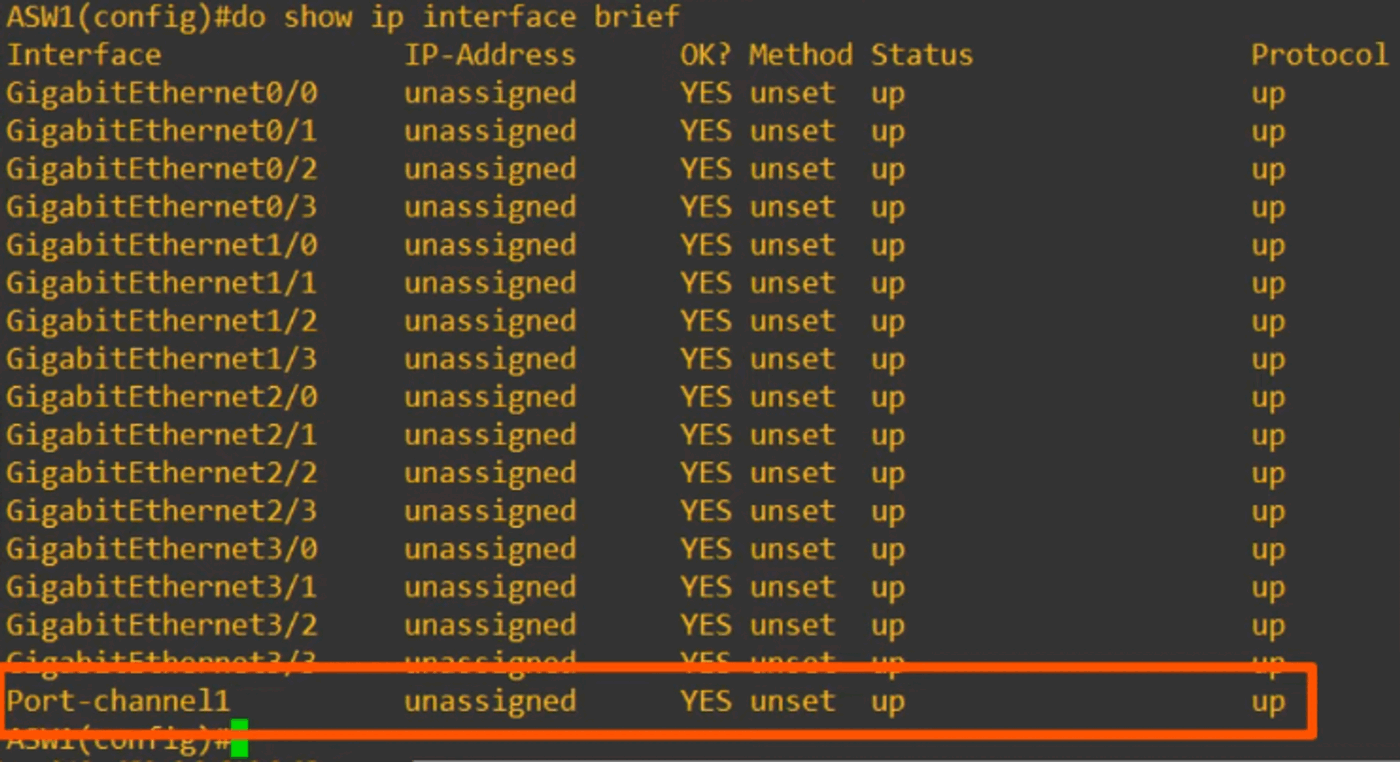
\includegraphics[keepaspectratio,alt={image}]{images/24-etherchannel/img-011.png}}
\end{figure}

The ``channel-group'' number has to MATCH for member INTERFACES on the
same SWITCH.

It DOESN'T have to MATCH the ``channel-group'' number on the OTHER
SWITCH!

(channel-group 1 on AWS1 can form an ETHERCHANNEL with channel-group 2
on DSW1)

\section{LACP Configuration}\label{lacp-configuration}

\begin{figure}
\centering
\pandocbounded{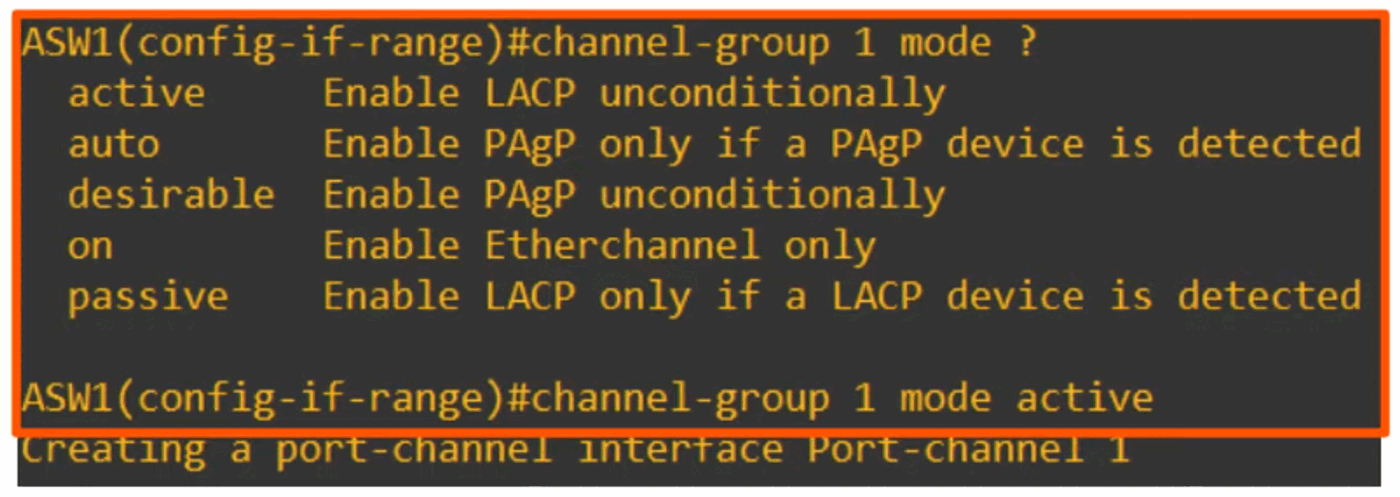
\includegraphics[keepaspectratio,alt={image}]{images/24-etherchannel/img-012.png}}
\end{figure}

NOTE that ``active'' and ``passive'' are the ONLY available modes for
LACP

\begin{figure}
\centering
\pandocbounded{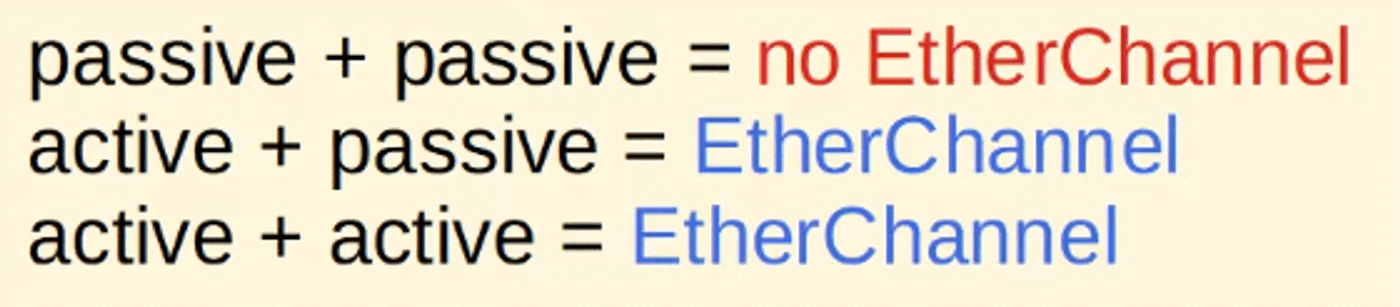
\includegraphics[keepaspectratio,alt={image}]{images/24-etherchannel/img-013.png}}
\end{figure}

LACP negotiations for form an ETHERCHANNEL

The ``channel-group'' number has to MATCH for member INTERFACES on the
same SWITCH.

It DOESN'T have to MATCH the ``channel-group'' number on the OTHER
SWITCH!

(channel-group 1 on AWS1 can form an ETHERCHANNEL with channel-group 2
on DSW1)

\section{Static EtherChannel
Configuration}\label{static-etherchannel-configuration}

\begin{figure}
\centering
\pandocbounded{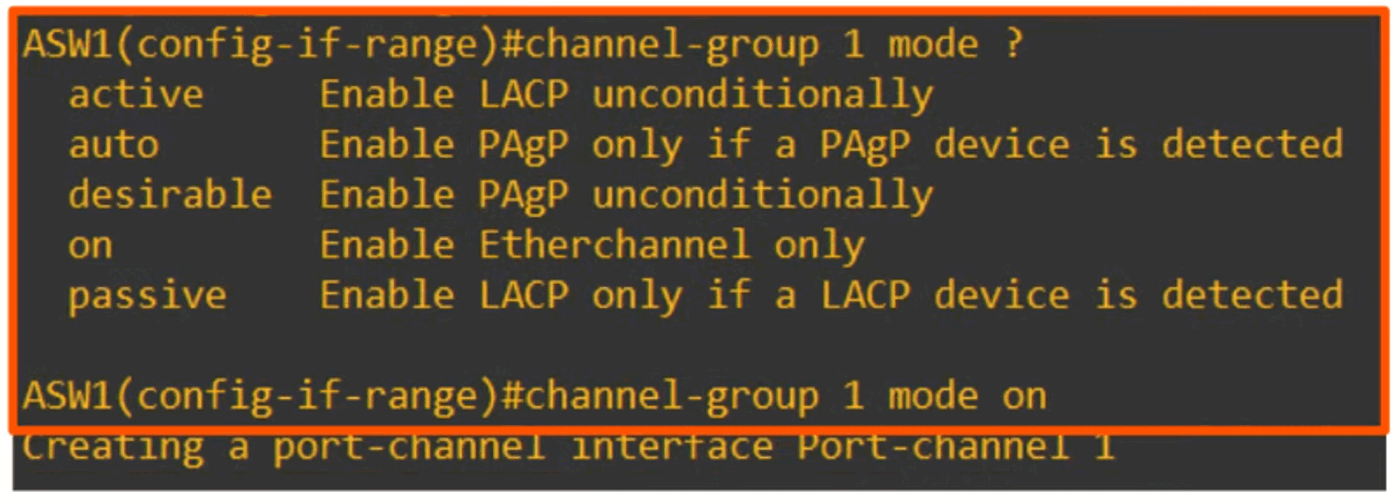
\includegraphics[keepaspectratio,alt={image}]{images/24-etherchannel/img-014.png}}
\end{figure}

NOTE that ``on'' is the ONLY available mode for STATIC ETHERCHANNEL

ON mode only works with ON Mode

ON + desirable = DOES NOT WORK)

ON + active = DOES NOT WORK

\section{How to Manually Configure the Negotiation
Protocol}\label{how-to-manually-configure-the-negotiation-protocol}

\begin{figure}
\centering
\pandocbounded{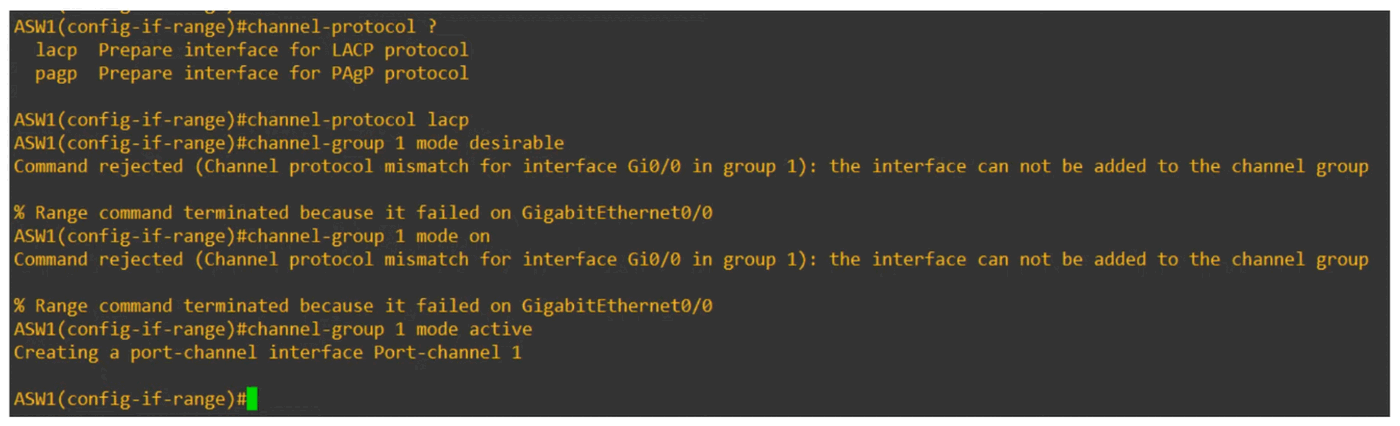
\includegraphics[keepaspectratio,alt={image}]{images/24-etherchannel/img-015.png}}
\end{figure}

\section{Two Options}\label{two-options}

\begin{itemize}
\tightlist
\item
  LACP Protocol
\item
  PAgP Protocol
\end{itemize}

(Above shows a protocol mismatch error because LACP does not support
``desirable'' - only PAgP does)

(``channel-group 1 mode active'' works because LACP supports ``active'')

\section{After Configuring the EtherChannel
Mode}\label{after-configuring-the-etherchannel-mode}

\section{Configuring the Port
Interface}\label{configuring-the-port-interface}

\begin{figure}
\centering
\pandocbounded{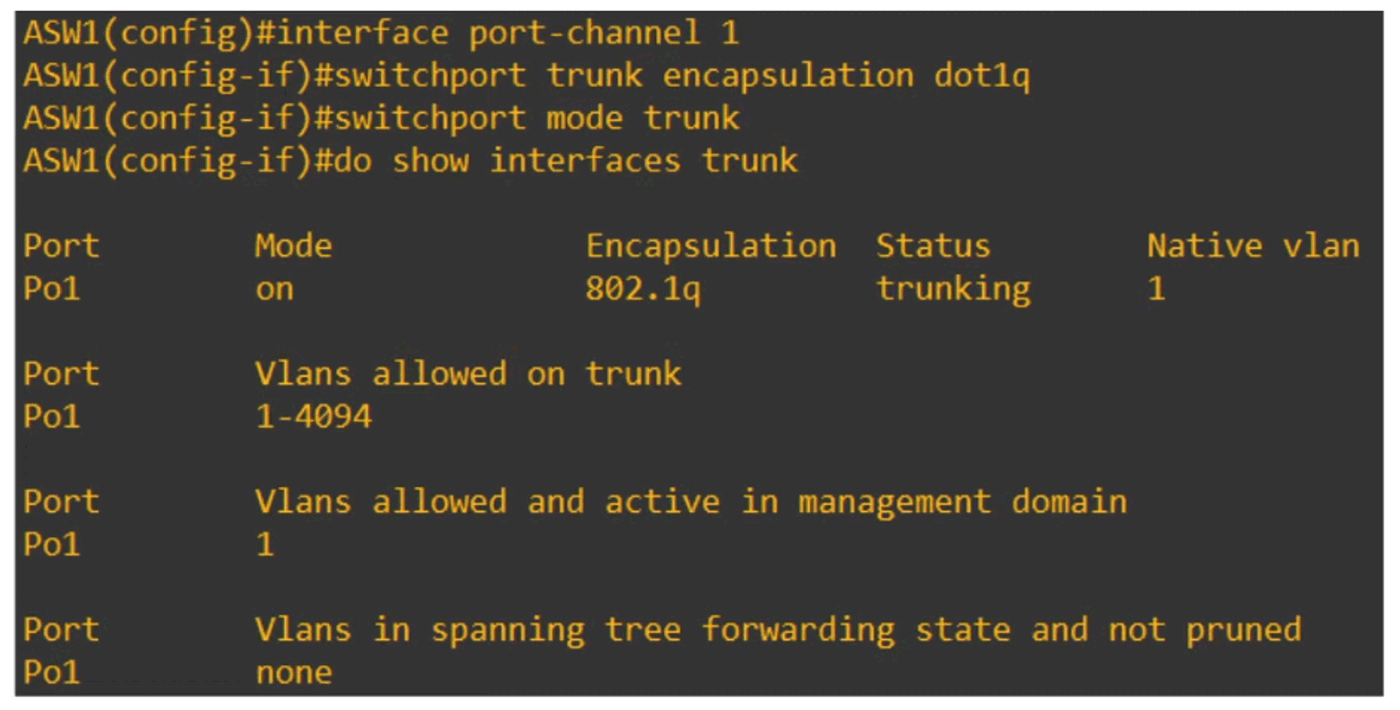
\includegraphics[keepaspectratio,alt={image}]{images/24-etherchannel/img-016.png}}
\end{figure}

``show running-config'' shows ``interface Port-channel1'' in the
configuration

\begin{figure}
\centering
\pandocbounded{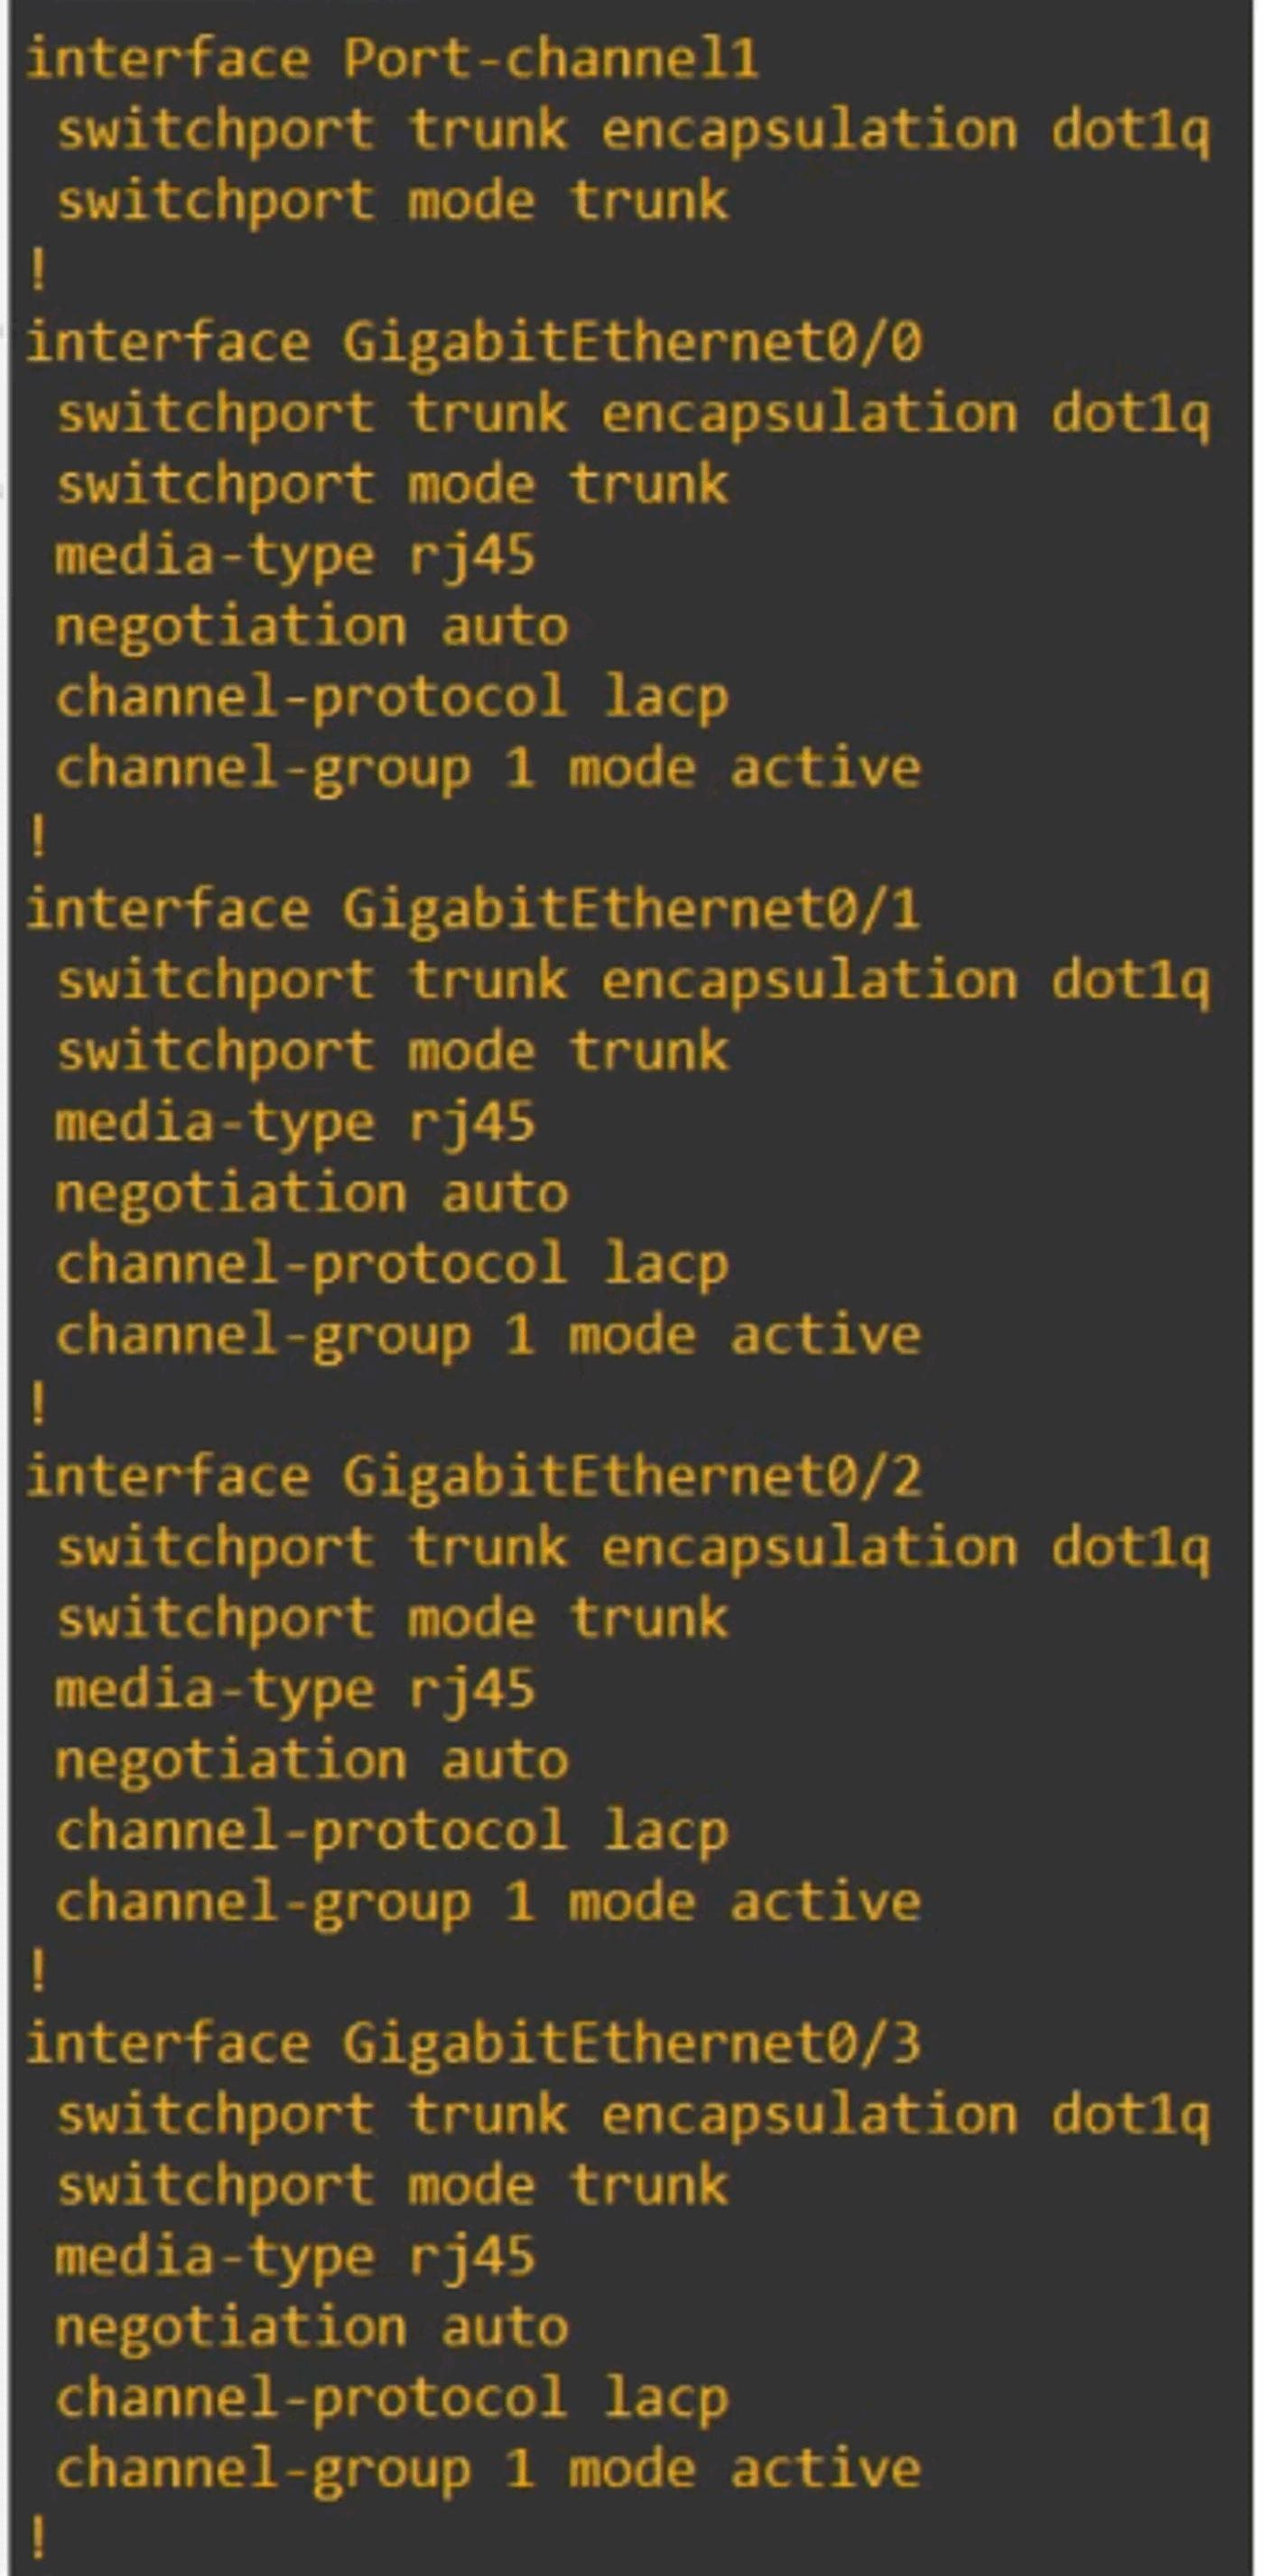
\includegraphics[keepaspectratio,alt={image}]{images/24-etherchannel/img-017.png}}
\end{figure}

NOTE the PHYSICAL INTERFACES (g0/0-g0/3) were auto-configured by the
Port-channel1 configuration!

\section{Important Notes About EtherChannel
Configuration}\label{important-notes-about-etherchannel-configuration}

\begin{itemize}
\tightlist
\item
  Member INTERFACES must have matching CONFIGURATIONS

  \begin{itemize}
  \tightlist
  \item
    Same DUPLEX (Full / Half)
  \item
    Same SPEED
  \item
    Same SWITCHPORT mode (Access / Trunk)
  \item
    Same allowed VLANs / Native VLAN (for TRUNK interfaces)
  \end{itemize}
\item
  If an INTERFACE's configurations do NOT MATCH the others, it will be
  EXCLUDED from the ETHERCHANNEL
\end{itemize}

\section{Verifying Status of
EtherChannel}\label{verifying-status-of-etherchannel}

``show etherchannel summary''

\begin{figure}
\centering
\pandocbounded{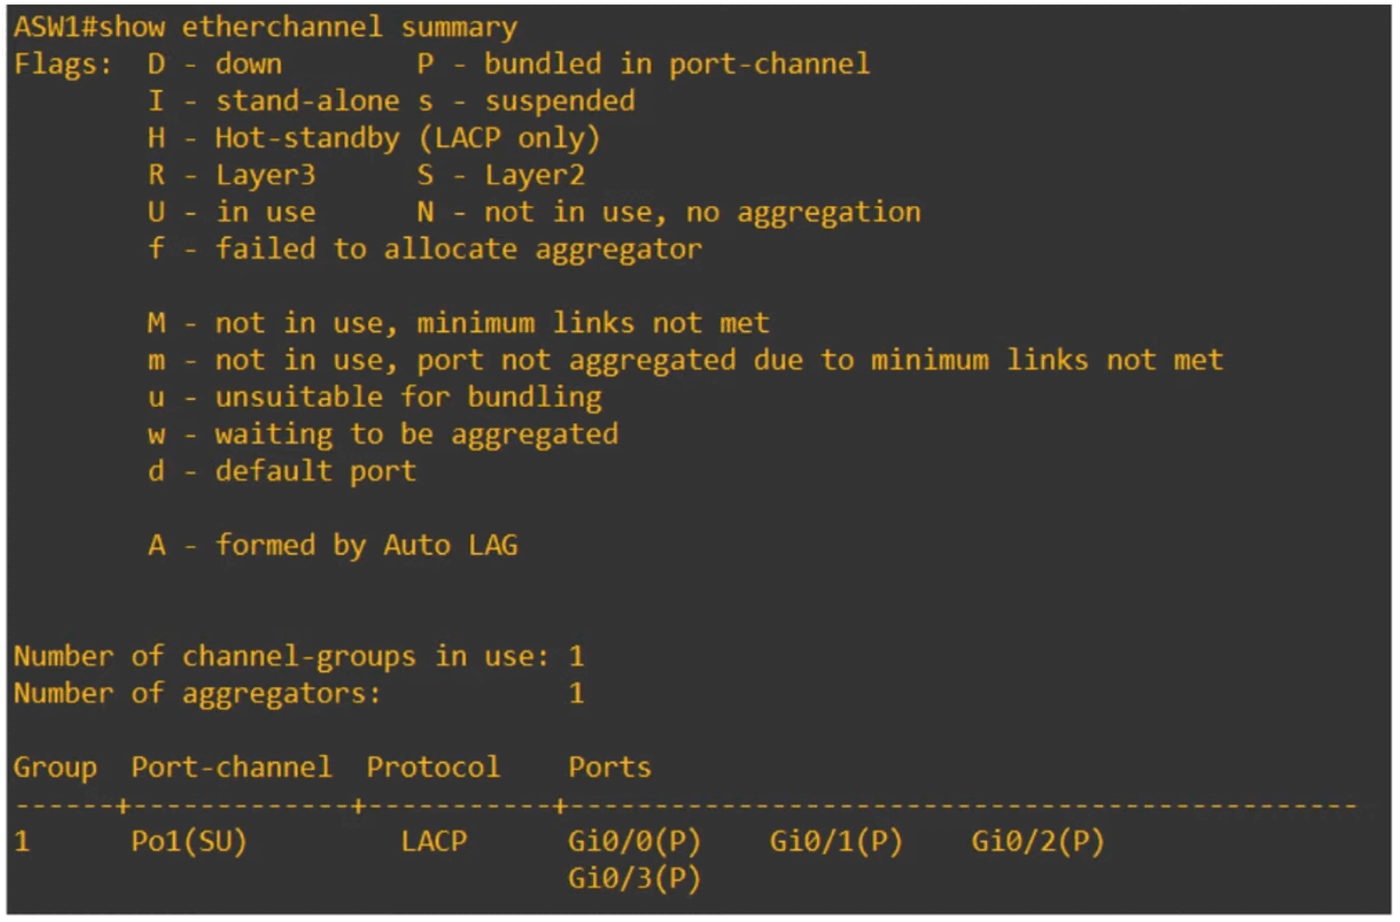
\includegraphics[keepaspectratio,alt={image}]{images/24-etherchannel/img-018.png}}
\end{figure}

NOTE information at bottom. (''SU'' means S - Layer2 + U - in use)

Protocol = What protocol the Etherchannel is using (in this case, LACP)

``Ports'' = the list of interfaces in the EtherChannel (P = bundled in
port-channel)

\section{Other Flags}\label{other-flags}

\begin{figure}
\centering
\pandocbounded{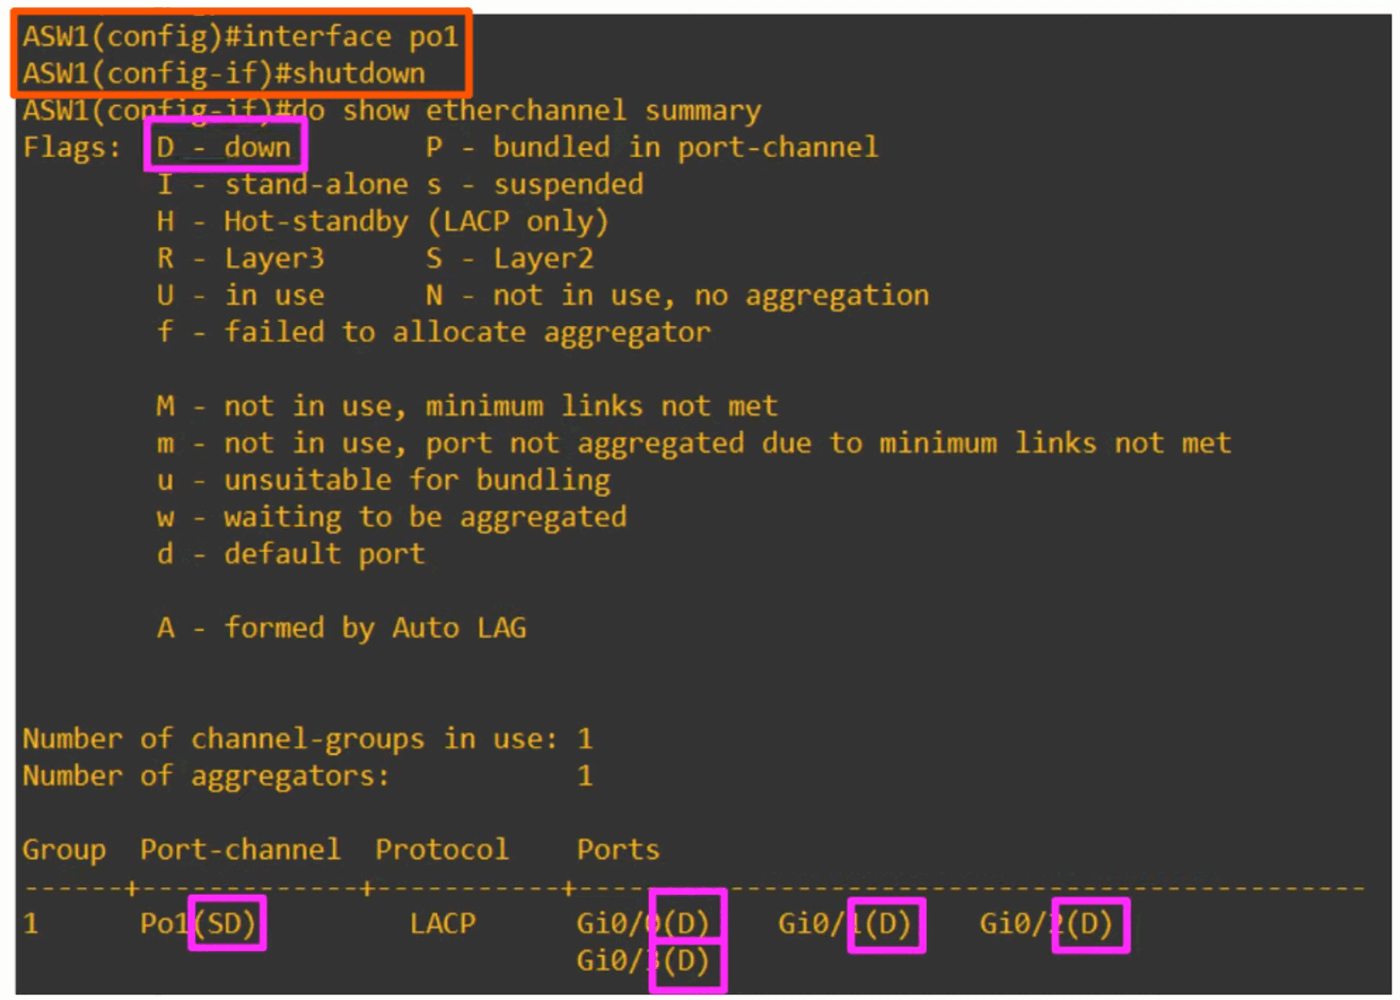
\includegraphics[keepaspectratio,alt={image}]{images/24-etherchannel/img-019.png}}
\end{figure}

``D'' = Down

\begin{figure}
\centering
\pandocbounded{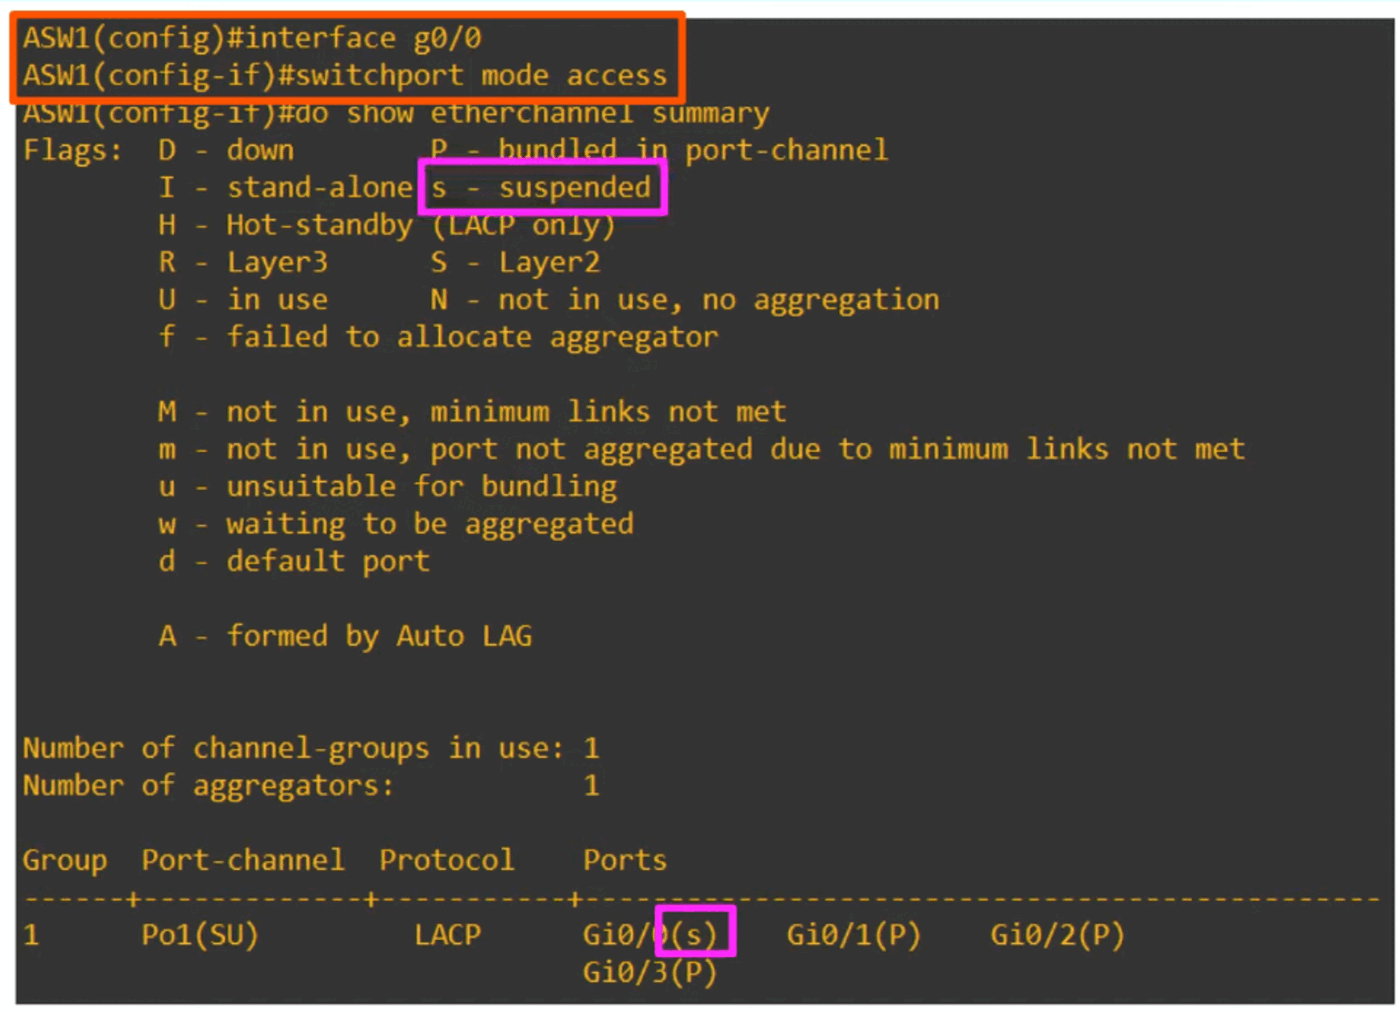
\includegraphics[keepaspectratio,alt={image}]{images/24-etherchannel/img-020.png}}
\end{figure}

Changing one of the Member interfaces using ``switchport mode access''
has made it different than the other members so it is now appearing as
``s'' = suspended

Another useful command

``show etherchannel port-channel''

\begin{figure}
\centering
\pandocbounded{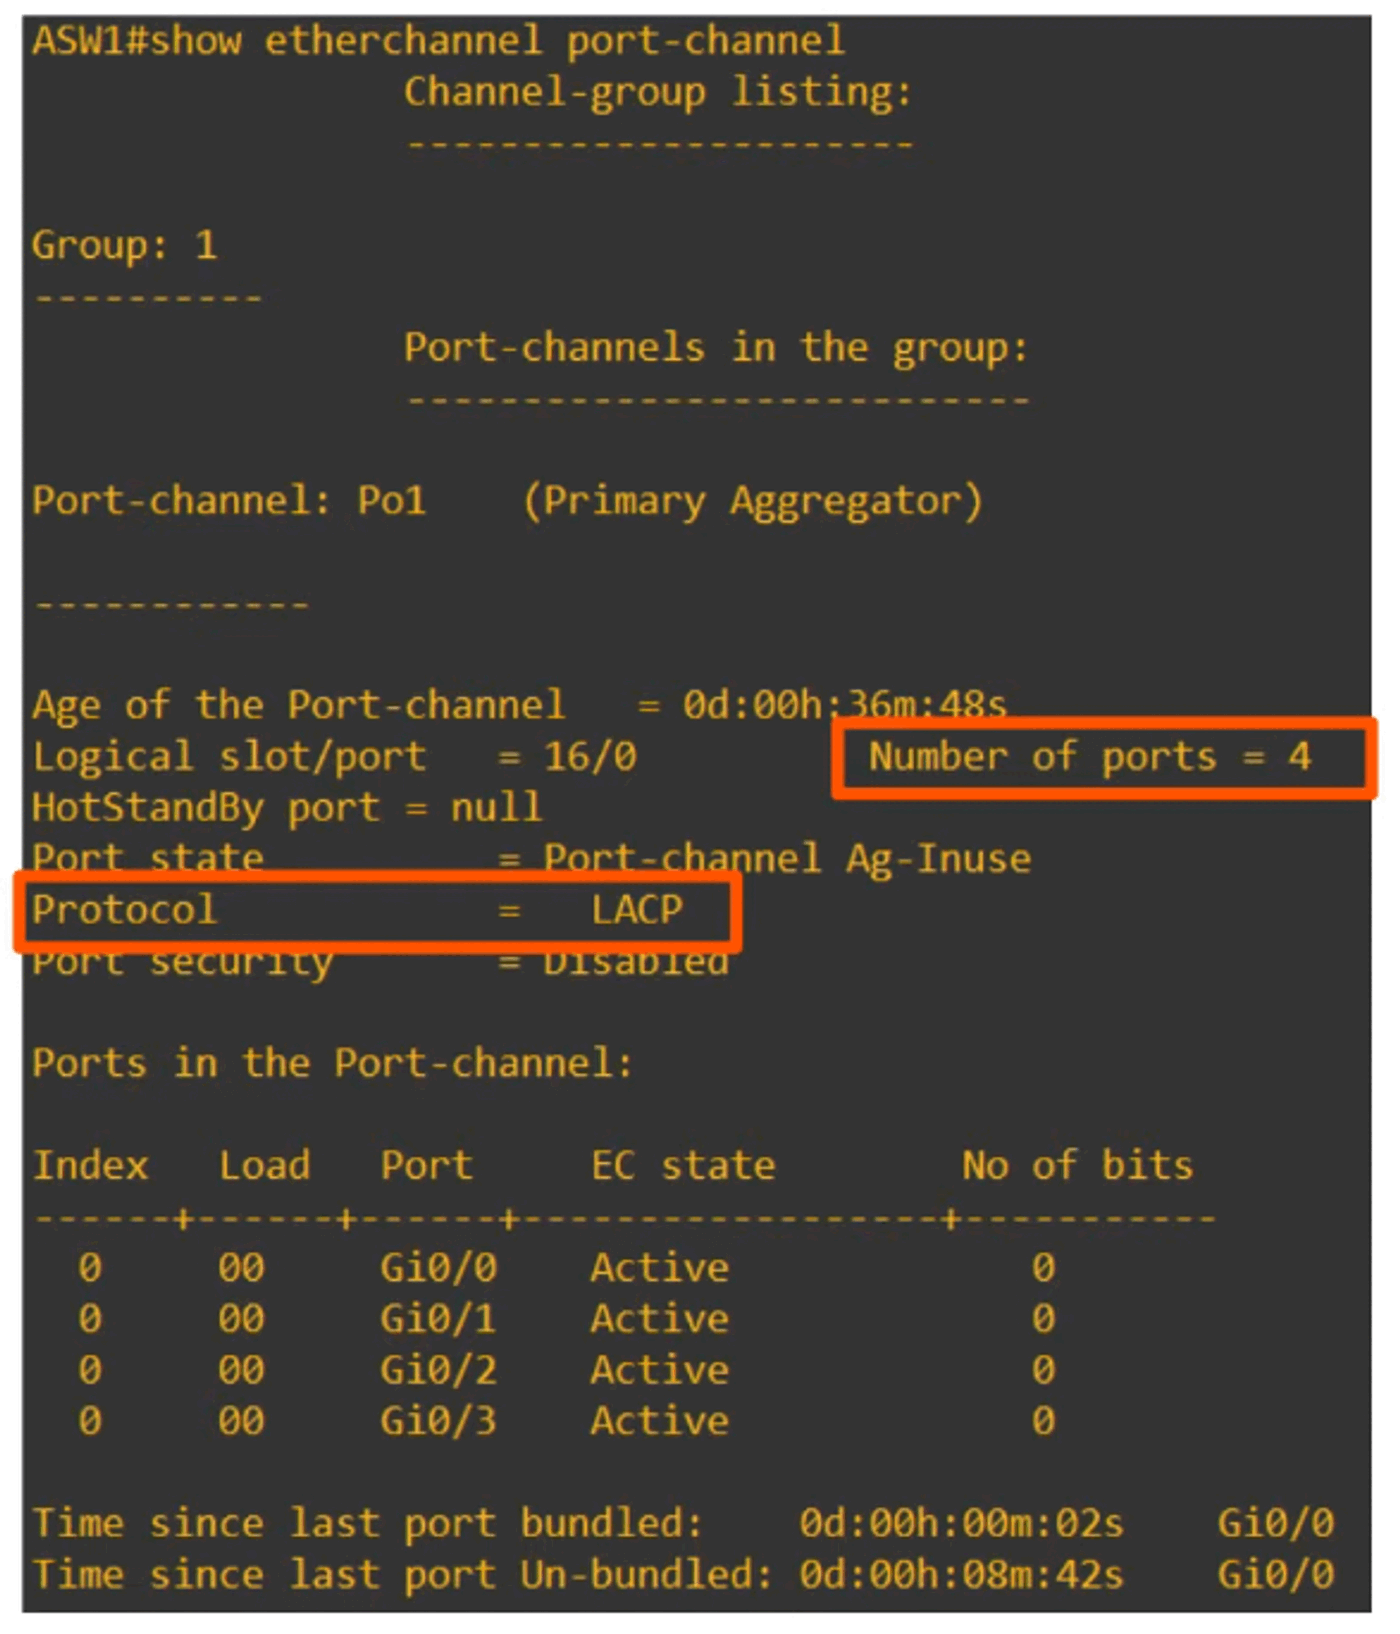
\includegraphics[keepaspectratio,alt={image}]{images/24-etherchannel/img-021.png}}
\end{figure}

``show spanning-tree'' will show the single EtherChannel port interface

\begin{figure}
\centering
\pandocbounded{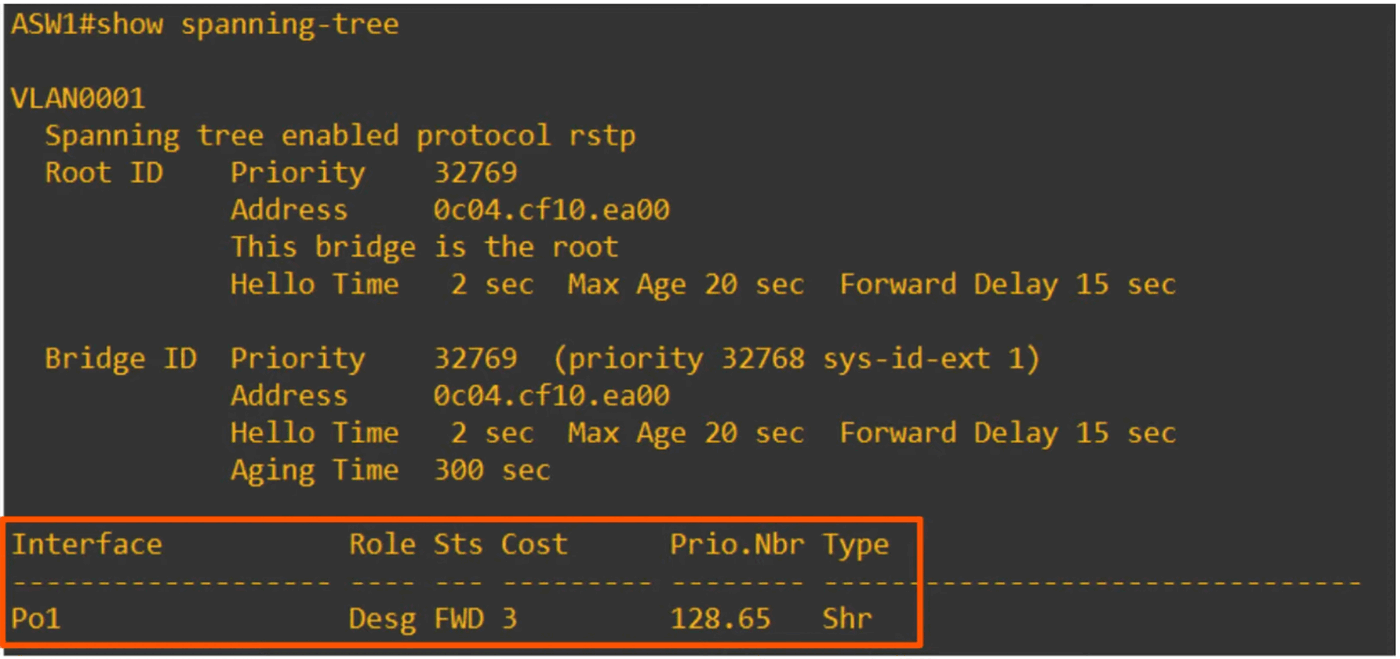
\includegraphics[keepaspectratio,alt={image}]{images/24-etherchannel/img-022.png}}
\end{figure}

\section{Layer 3 EtherChannels}\label{layer-3-etherchannels}

\begin{figure}
\centering
\pandocbounded{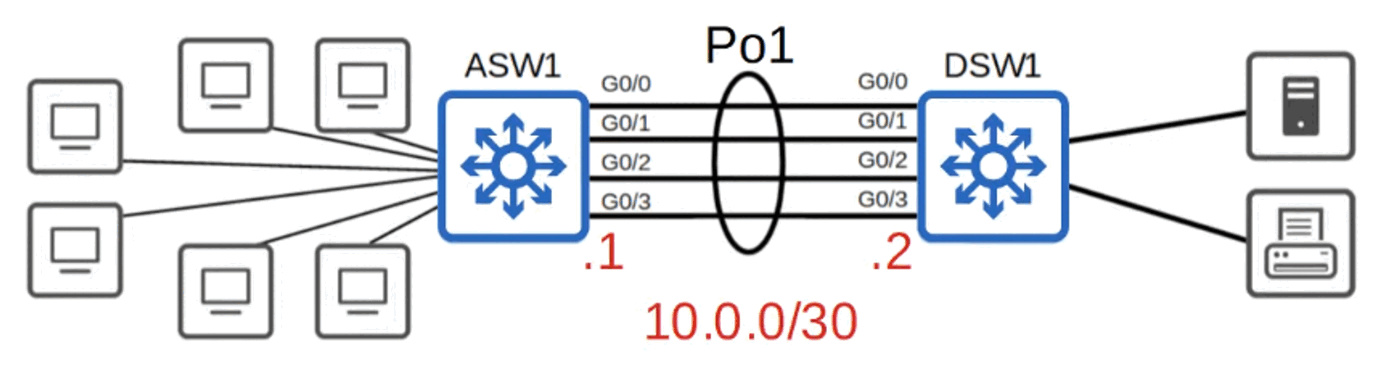
\includegraphics[keepaspectratio,alt={image}]{images/24-etherchannel/img-023.png}}
\end{figure}

HOW TO CONFIGURE A LAYER 3 ETHERCHANNEL (from a clean configuration)

\begin{figure}
\centering
\pandocbounded{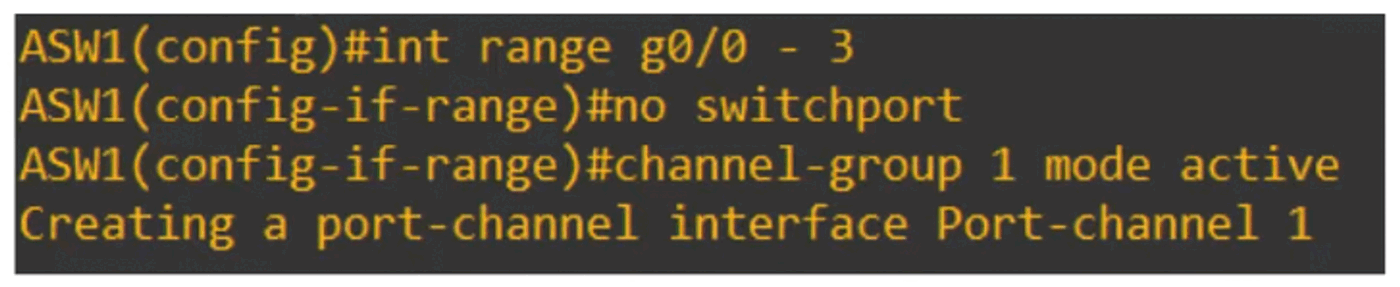
\includegraphics[keepaspectratio,alt={image}]{images/24-etherchannel/img-024.png}}
\end{figure}

``show running-config''

\begin{figure}
\centering
\pandocbounded{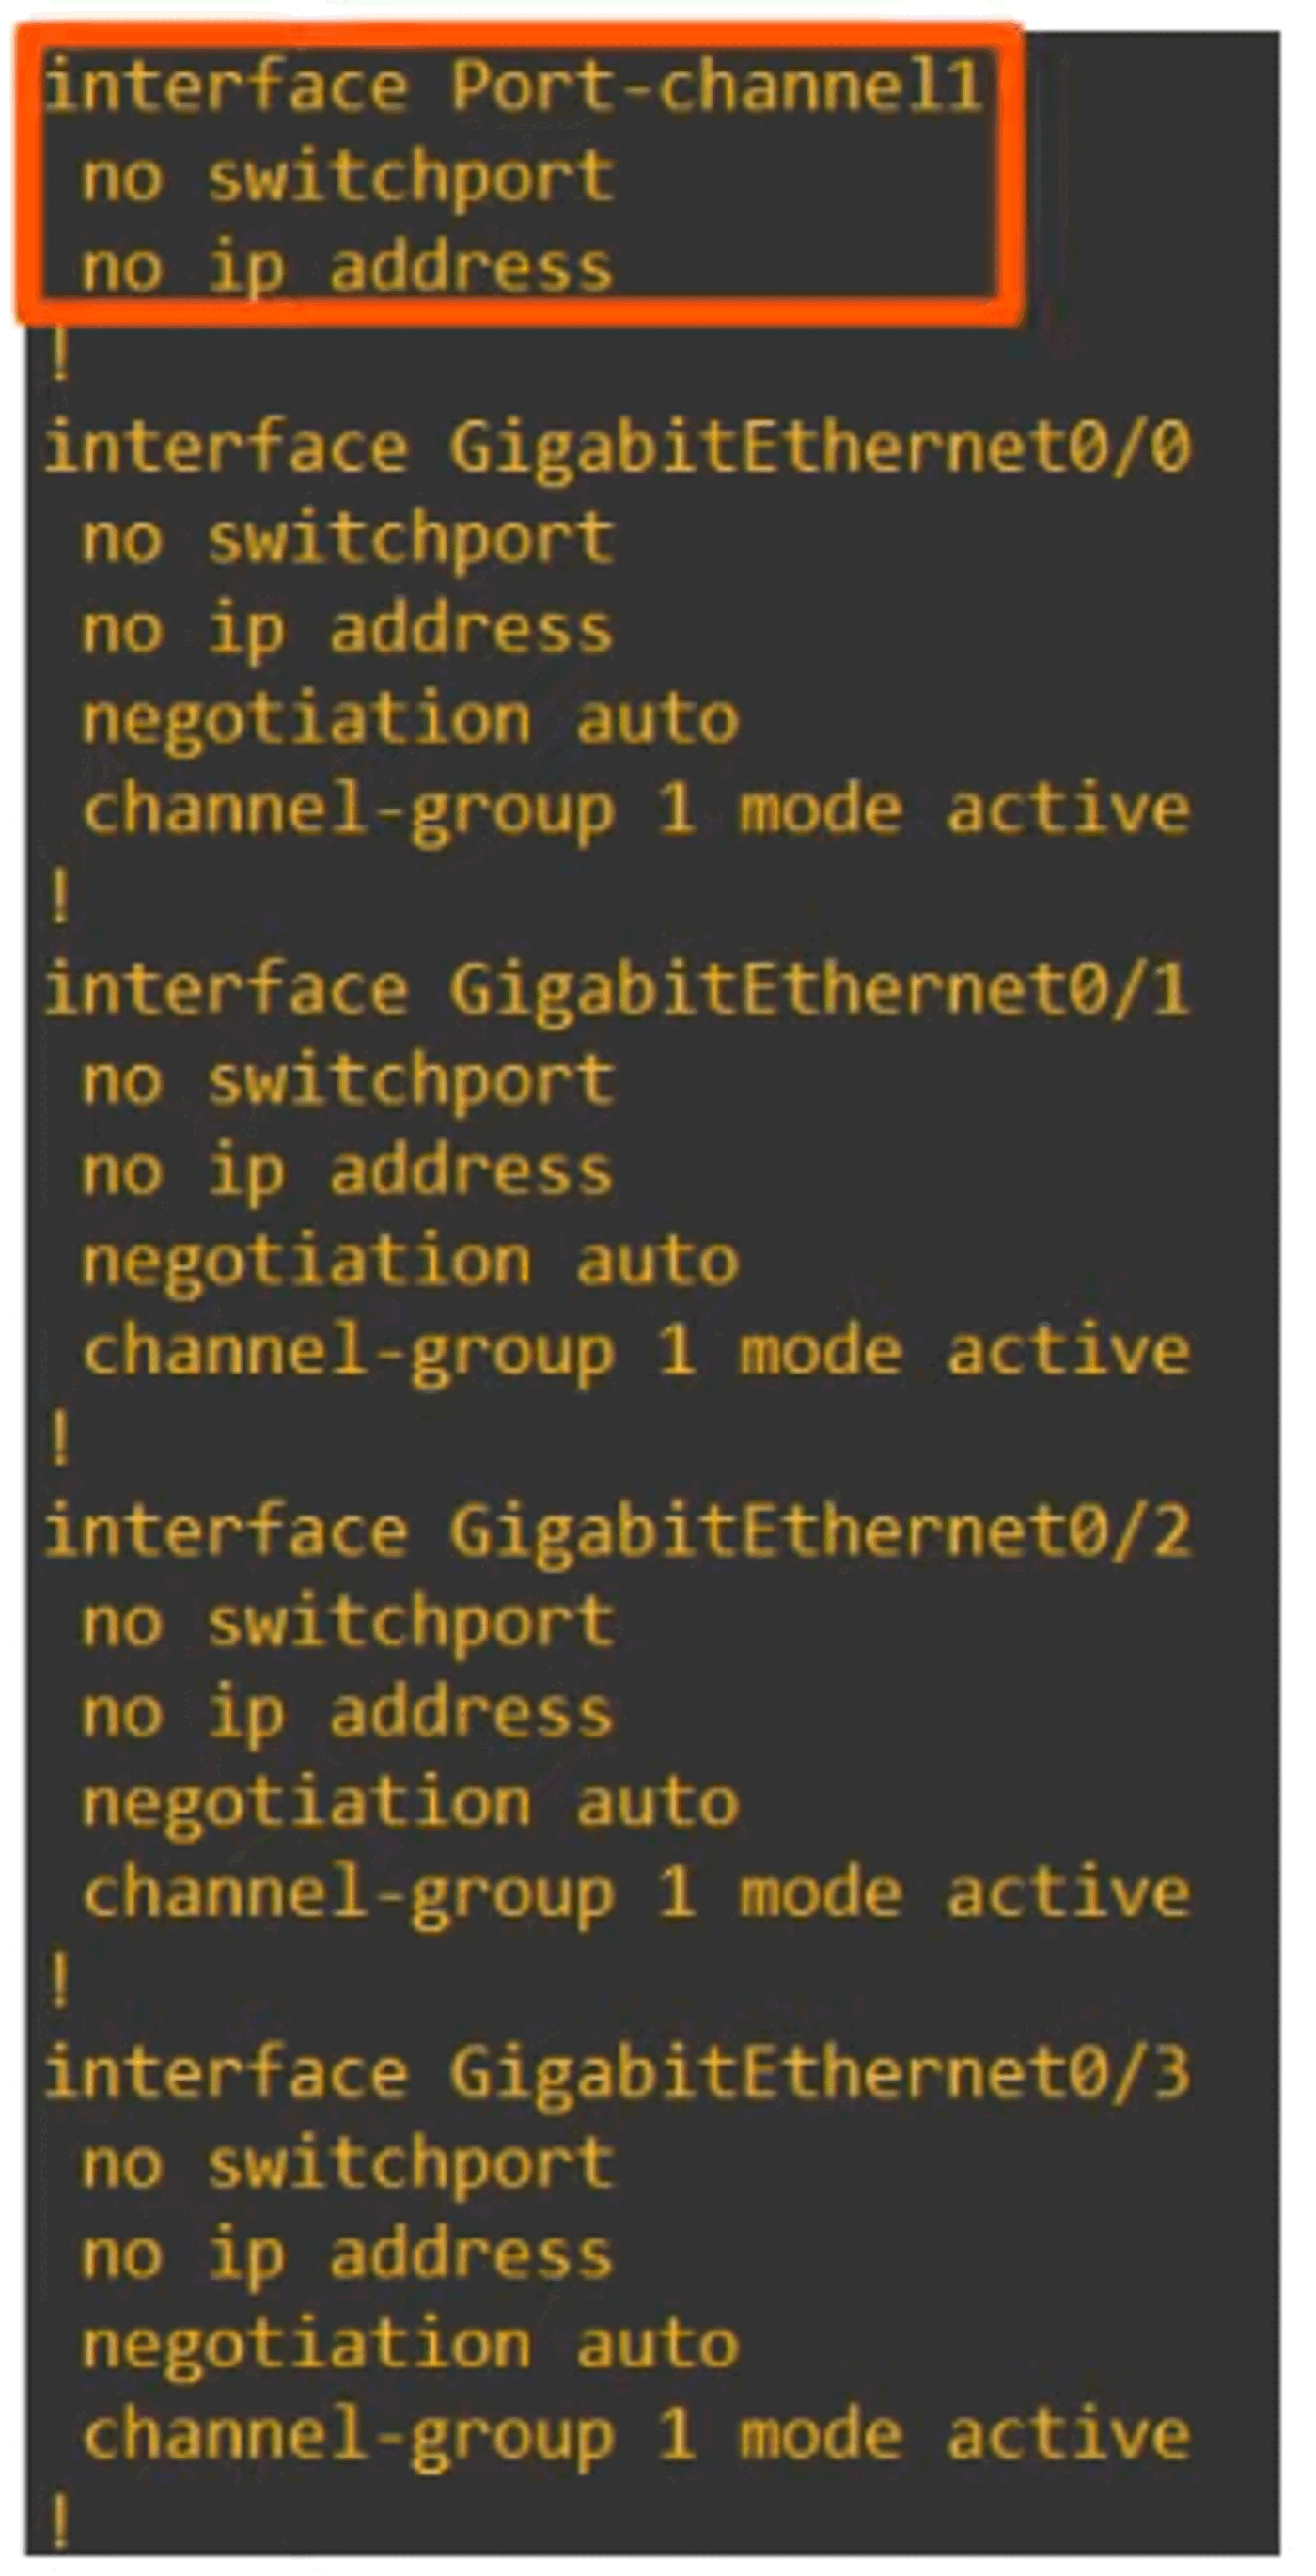
\includegraphics[keepaspectratio,alt={image}]{images/24-etherchannel/img-025.png}}
\end{figure}

NOTE : No SWITCHPORT and NO IP INTERFACE.

Where do we configure the IP Address? Directly on the PORT INTERFACE !

\begin{figure}
\centering
\pandocbounded{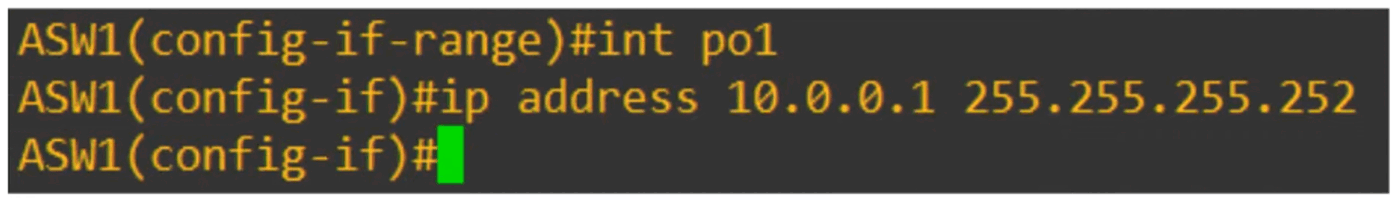
\includegraphics[keepaspectratio,alt={image}]{images/24-etherchannel/img-026.png}}
\end{figure}

\begin{figure}
\centering
\pandocbounded{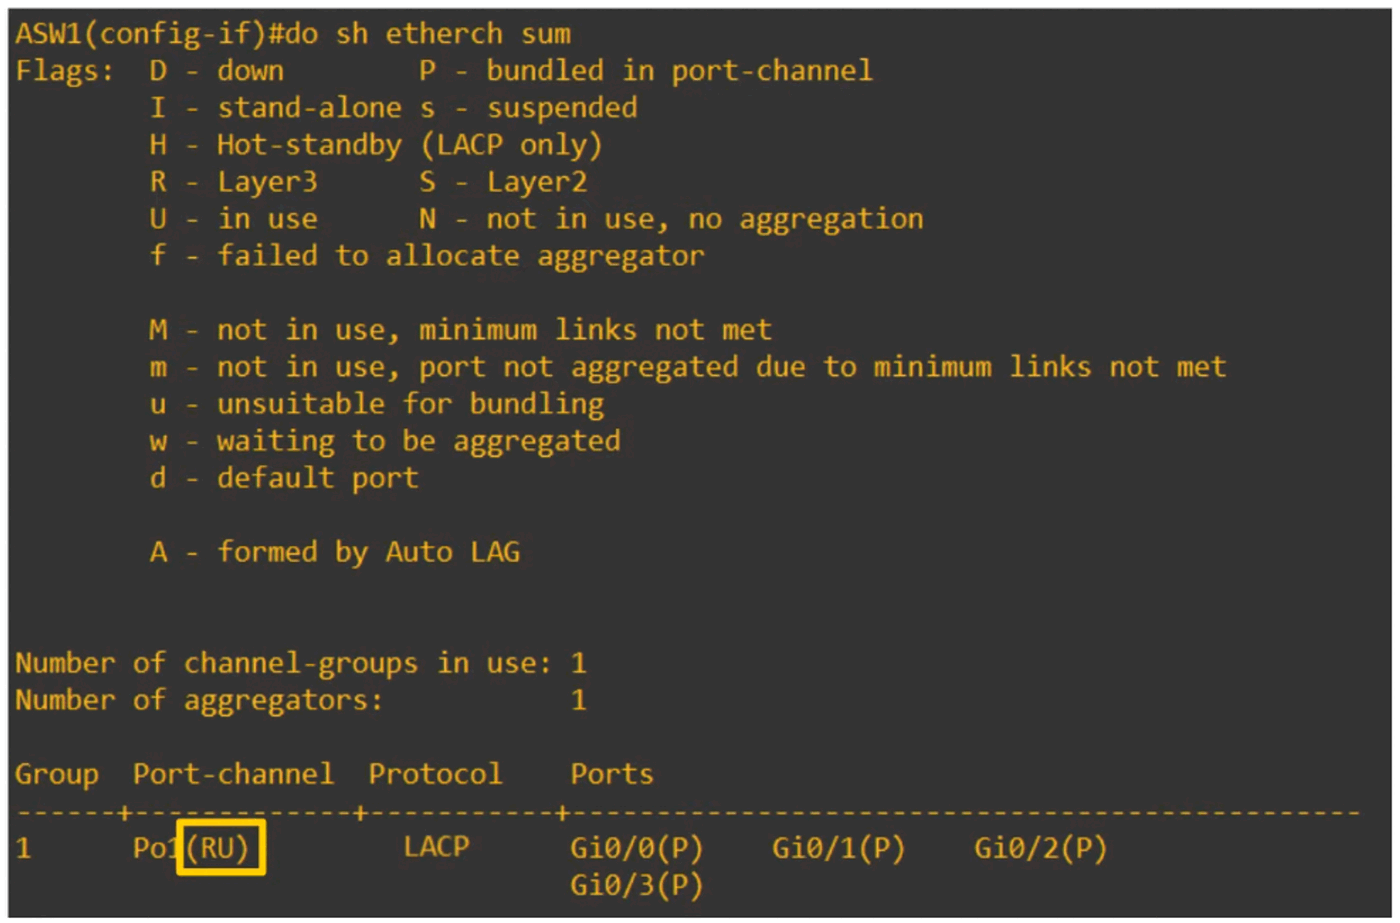
\includegraphics[keepaspectratio,alt={image}]{images/24-etherchannel/img-027.png}}
\end{figure}

(''RU'' - ``R'' = Layer 3, ``U'' = in use)

\begin{figure}
\centering
\pandocbounded{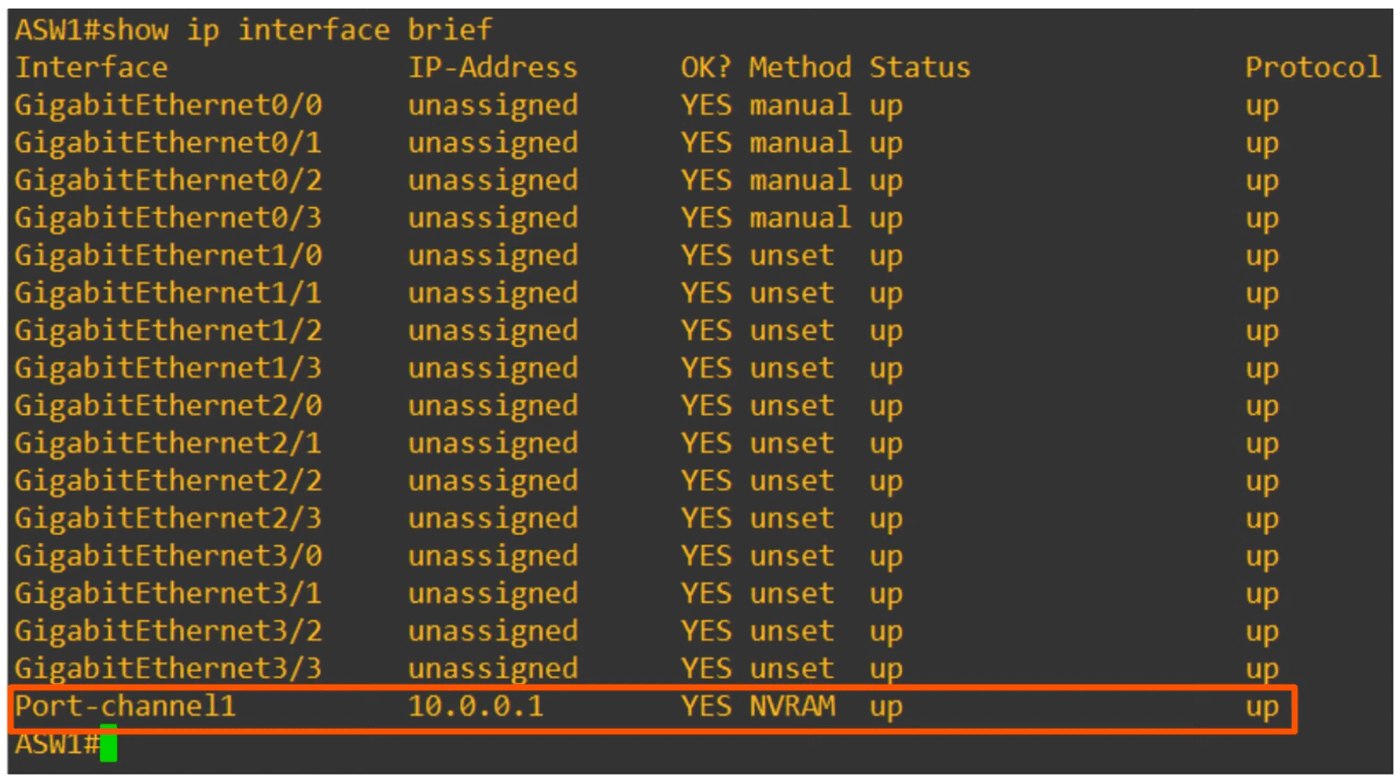
\includegraphics[keepaspectratio,alt={image}]{images/24-etherchannel/img-028.png}}
\end{figure}

COMMANDS LEARNED IN THIS CHAPTER

\begin{lstlisting}
SW(config) port-channel load-balance *mode*
\end{lstlisting}

Configures the EtherChannel load-balancing method on a SWITCH

\begin{lstlisting}
SW# show etherchannel load-balance
\end{lstlisting}

Displays information about the load-balancing settings

\begin{lstlisting}
SW(config-if)# channel-group *number* mode {desirable | auto | active | passive | on}
\end{lstlisting}

Configures an interface to be PART of an EtherChannel

\begin{lstlisting}
SW# show etherchannel summary
\end{lstlisting}

Displays a summary of EtherChannels on a SWITCH

\begin{lstlisting}
SW# show etherchannel port-channel
\end{lstlisting}

Displays information about the virtual port-channel interfaces on a
SWITCH

\begin{figure}
\centering
\pandocbounded{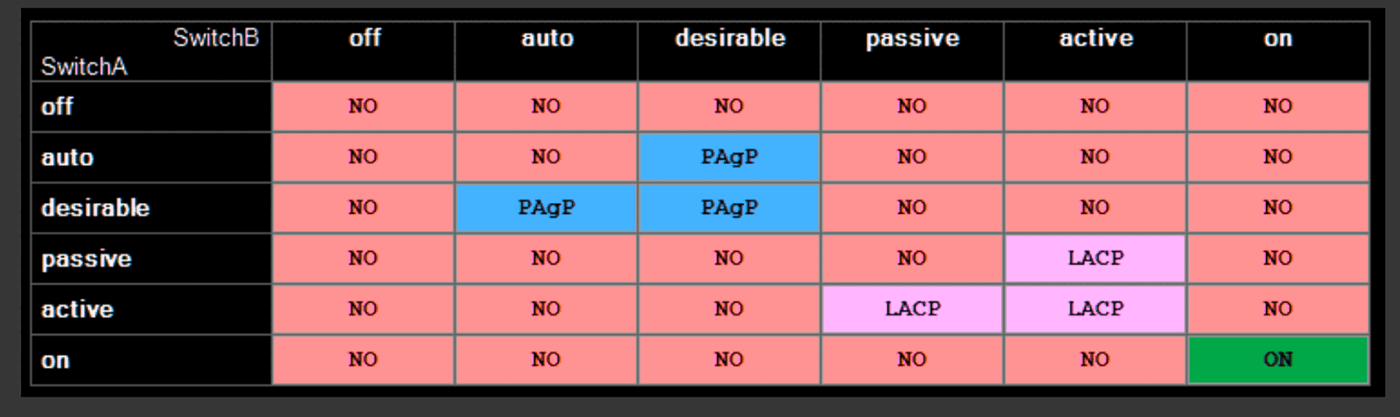
\includegraphics[keepaspectratio,alt={image}]{images/24-etherchannel/img-029.png}}
\end{figure}
